\documentclass[12pt]{article}

\usepackage[a4paper, left=2cm, right=2cm]{geometry} % A4 paper size and thin margins

\usepackage{xcolor} % Required for specifying custom colours
\definecolor{grey}{rgb}{0.8,0.8,1} % Colour of the box surrounding the title

\usepackage[T1]{fontenc}
\usepackage[utf8]{inputenc} % Output font encoding for international characters
\usepackage[portuguese]{babel}
\usepackage{graphicx}
\usepackage[sfdefault]{ClearSans} % Use the Clear Sans font (sans serif)
%\usepackage{XCharter} % Use the XCharter font (serif)
\usepackage{fancyhdr}
\usepackage{listings}
\usepackage{xcolor}
\usepackage{float}

\definecolor{codegreen}{rgb}{0,0.6,0}
\definecolor{codegray}{rgb}{0.5,0.5,0.5}
\definecolor{codepurple}{rgb}{0.58,0,0.82}
\definecolor{backcolour}{rgb}{0.95,0.95,0.92}

\lstdefinestyle{mystyle}{
    backgroundcolor=\color{backcolour},
    commentstyle=\color{codegreen},
    keywordstyle=\color{magenta},
    numberstyle=\tiny\color{codegray},
    stringstyle=\color{codepurple},
    basicstyle=\ttfamily\footnotesize,
    breakatwhitespace=false,
    breaklines=true,
    captionpos=b,
    keepspaces=true,
    numbers=left,
    numbersep=5pt,
    showspaces=false,
    showstringspaces=false,
    showtabs=false,
    tabsize=2
}

\lstset{style=mystyle}

\fancyhf{}
\pagestyle{fancy}
\rfoot{\thepage\hspace{1pt}}
\begin{document}

\begin{titlepage}

	\colorbox{grey}{
		\parbox[t]{0.93\textwidth}{ % Outer full width box
			\parbox[t]{0.91\textwidth}{ % Inner box for inner right text margin
				\raggedleft
				\fontsize{50pt}{80pt}\selectfont
				\vspace{0.5cm}

				Relatório do Curso de Prática Simulada\\


				\vspace{0.5cm}
			}
		}
	}
	\vfill

	\parbox[t]{0.93\textwidth}{
		\raggedleft
		\large
		{\Large Diogo Valério}\\[4pt]
		11PSI nº4\\
		Escola Secundária António Damásio\\[4pt]
		\hfill\rule{0.6\linewidth}{1pt}
	}
\end{titlepage}


\tableofcontents
\newpage

\section{Introdução}
Este relatório foi realizado no âmbito do curso de prática simulada facultado pela \textbf{ANPRI} (Associação Nacional Professores de Informática), a que fomos submetidos no lugar da Formação em Contexto de Trabalho devido à pandemia de Covid-19 a que estamos a passar de momento.

O curso frequentado foi o \textbf{Curso 2: Técnicas básicas de escrita de páginas dinâmicas em PHP} e decorreu de 19 de maio a 8 de julho, mas, devido a problemas técnicos na plataforma e também a ataques de  \textit{Denial of Service}(também conhecido como DDOS) à plataforma, o decorrer normal do curso foi prejudicado, sendo que este acabou por ser movido para o servico \textit{Google Sites}.


\section{Caracterização do Curso}
\subsection{Objetivos do Curso}
No inicio os objetivos do curso foram bem delimitados como mostra a figura seguinte:

\begin{figure}[h]
        \centering
        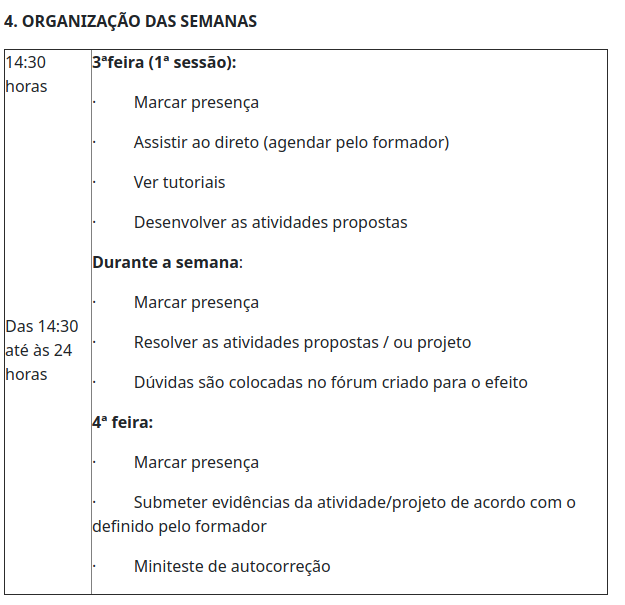
\includegraphics[width=0.45\linewidth]{cal.png}
        \caption{Menu de Interação}
        \label{fig:menu1}
\end{figure}


No entanto estes não foram cumpridos em qualquer aspecto:
\begin{list}{•}{•}
\item Não existiu nenhuma forma de marcar presença no dia 19 (mostrava apenas uma marcação de presença para dia 20),
e no dia seguinte foi introduzida

\item Não houve qualquer interação no primeiro dia de curso por parte do formador (Prof. Carlos)
\end{list}


\end{document}
